\documentclass[a4paper]{article}
\usepackage[a4paper,margin=0mm]{geometry}
\usepackage{fontspec}
\usepackage{unicode-math}
\usepackage{tikz}
\usetikzlibrary{fit,calc,positioning}
\usepackage[table]{xcolor}
\usepackage[absolute]{textpos}
\usepackage{array}

\setmainfont{Libertinus Serif}
\setsansfont{Libertinus Sans}
\setmathfont{Libertinus Math}

\definecolor{accent}{HTML}{F46530}
\definecolor{badge}{HTML}{FFBDA5}
\definecolor{ink}{HTML}{2A2E30}

\setlength{\TPHorizModule}{1mm}
\setlength{\TPVertModule}{1mm}
\setlength{\parindent}{0pt}
\pagestyle{empty}

\newcommand{\topicheader}[2]{%
\begin{textblock*}{194mm}(16mm,10mm)
\begin{tikzpicture}
\node[fill=accent,text=white,font=\sffamily\bfseries\fontsize{13}{13}\selectfont,
      minimum width=9mm,minimum height=9mm,inner sep=0pt] at (4.5mm,-4.5mm) {#1};
\node[font=\sffamily\bfseries\fontsize{15}{16}\selectfont,text=ink,anchor=west] at (12mm,-4.5mm) {#2};
\end{tikzpicture}
\end{textblock*}
\begin{textblock*}{194mm}(16mm,22.5mm)

\begin{tikzpicture}
\fill[accent] (0,0) rectangle (194mm,0.5mm);
\end{tikzpicture}
\end{textblock*}
}

\newcommand{\pagekicker}[1]{%
\begin{textblock*}{100mm}(16mm,25.5mm)
\begin{tikzpicture}
\node[fill=ink,text=white,font=\sffamily\bfseries\fontsize{8}{8}\selectfont,
      inner sep=2.2pt,rounded corners=1pt] {\MakeUppercase{#1}};
\end{tikzpicture}
\end{textblock*}
}

\newcommand{\pagefooter}[1]{%
\begin{textblock*}{194mm}(8mm,286.41mm)
  
\begin{tikzpicture}
    \fill[accent] (0,0) rectangle (194mm,0.6mm);
  \end{tikzpicture}
\end{textblock*}
\begin{textblock*}{63.59mm}(8mm,288.27mm)
  {\sffamily\bfseries\color{accent}\fontsize{13}{16}\selectfont SAT 1200+}
\end{textblock*}
\begin{textblock*}{10mm}(188mm,288.27mm)
  \centering{\sffamily\color{accent}\fontsize{14}{16}\selectfont #1}
\end{textblock*}
}

\newcommand{\cardbg}[4]{%
\begin{textblock*}{#3mm}(#1mm,#2mm)
\begin{tikzpicture}
\fill[badge!22,rounded corners=3mm] (0,0) rectangle (#3mm,-#4mm);
\end{tikzpicture}
\end{textblock*}%
}

\newcommand{\pill}[3]{%
\begin{textblock*}{160mm}(#1mm,#2mm)
\begin{tikzpicture}
\node[fill=accent,text=white,anchor=north west,font=\sffamily\bfseries\fontsize{10}{10}\selectfont,
      rounded corners=8pt,inner xsep=5mm,inner ysep=1.8mm] at (0,0) {QOIDA ~\textperiodcentered~ #3};
\end{tikzpicture}
\end{textblock*}%
}

\arrayrulecolor{accent}
\setlength{\arrayrulewidth}{0.7pt}
\renewcommand{\arraystretch}{1.5}

\begin{document}

\topicheader{4}{Ishorali sonlar}
\pagekicker{Formula sheet}
\pagefooter{41}
\mbox{}%

% ================= CARD 1: Musbat/manfiy va modul (y: 33-88) =================
\cardbg{16}{33}{178}{55}
\pill{26}{36}{Musbat/manfiy va modul}

\begin{textblock*}{158mm}(26mm,48mm)
{\fontsize{11}{14}\selectfont\setlength{\tabcolsep}{4pt}
\begin{tabular}{|>{\centering\arraybackslash}p{32mm}|>{\centering\arraybackslash}p{54mm}|>{\centering\arraybackslash}p{54mm}|}
\hline
\rowcolor{accent}
{\color{white}\textbf{Son}} & {\color{white}\textbf{Modul}} & {\color{white}\textbf{Qarama-qarshi son}} \\ \hline
$7$ & $|7|=7$ & $-7$ \\ \hline
$-7$ & $|-7|=7$ & $7$ \\ \hline
$-12$ & $|-12|=12$ & $12$ \\ \hline
\end{tabular}}
\end{textblock*}

% ================= CARD 2: Qo'shish / ayirish (y: 94-164) =================
\cardbg{16}{94}{178}{70}
\pill{26}{97}{Qo'shish / ayirish}

\begin{textblock*}{158mm}(26mm,109mm)
{\fontsize{10.5}{13}\selectfont\color{ink}
Bir xil ishora: modullarni qo'shing, ishorani saqlang. Har xil ishora: kattasidan kichigini ayiring, kattaning ishorasini oling. Manfiyni ayirish -- musbatini qo'shish: $a-(-b)=a+b$.}
\end{textblock*}

\begin{textblock*}{158mm}(26mm,131mm)
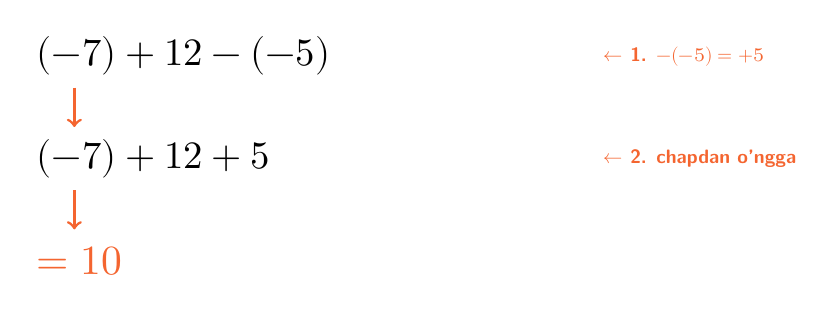
\begin{tikzpicture}[every node/.style={font=\fontsize{14}{14}\selectfont}]
\node[anchor=west] (l0) at (0,0) {$(-7)+12-(-5)$};
\node[anchor=west,font=\sffamily\bfseries\scriptsize,text=accent] at (72mm,0) {$\leftarrow$ 1. $-(-5)=+5$};

\node[anchor=west] (l1) at (0,-13mm) {$(-7)+12+5$};
\node[anchor=west,font=\sffamily\bfseries\scriptsize,text=accent] at (72mm,-13mm) {$\leftarrow$ 2. chapdan o'ngga};

\node[anchor=west,font=\sffamily\bfseries\fontsize{15}{15}\selectfont,text=accent] (l2) at (0,-26mm) {$=10$};

\foreach \y in {-4,-17}{
  \draw[accent,->,line width=1pt] (6mm,\y mm) -- (6mm,\y mm -5mm);
}
\end{tikzpicture}
\end{textblock*}

% ================= CARD 3: Ko'paytirish/bo'lish -- ishora qoidasi (left) / necha marta manfiy (right) (y: 170-225) =================
\cardbg{16}{170}{85}{55}
\pill{22}{173}{Ko'paytirish / bo'lish}

\begin{textblock*}{85mm}(22mm,189mm)
{\fontsize{11}{15}\selectfont
\begin{tabular}{|>{\centering\arraybackslash}p{30mm}|>{\centering\arraybackslash}p{30mm}|}
\hline
\rowcolor{accent}
{\color{white}\textbf{Ishoralar}} & {\color{white}\textbf{Natija}} \\ \hline
bir xil & $+$ \\ \hline
har xil & $-$ \\ \hline
\end{tabular}}
\end{textblock*}

\cardbg{109}{170}{85}{55}
\pill{115}{173}{Necha marta manfiy?}

\begin{textblock*}{85mm}(109mm,189mm)
\begin{center}
{\fontsize{12}{12}\selectfont $(-4)\times(-3)\div(-2)$}

\vspace{2mm}
{\fontsize{9.5}{11}\selectfont\color{ink} $(-4)\times(-3)=12$ (bir xil)}

{\fontsize{9.5}{11}\selectfont\color{ink} $12\div(-2)=-6$ (har xil)}

\vspace{1.5mm}
{\fontsize{13}{13}\selectfont\color{accent} $=-6$}
\end{center}
\end{textblock*}

% ================= CARD 4: Qavs ochish (y: 231-281) =================
\cardbg{16}{231}{178}{50}
\pill{26}{234}{Qavs ochish}

\begin{textblock*}{158mm}(26mm,243mm)
\begin{center}
{\fontsize{13}{15}\selectfont $-(a+b)=-a-b \qquad -(a-b)=-a+b$}
\end{center}
\end{textblock*}

\begin{textblock*}{158mm}(26mm,251mm)
\begin{tikzpicture}[every node/.style={font=\fontsize{13}{13}\selectfont}]
\node[anchor=west] (r0) at (0,0) {$-(7-4)+3$};
\node[anchor=south,font=\sffamily\bfseries\fontsize{8}{8}\selectfont,text=accent] at (41mm,4mm) {$-(7-4)=-7+4$};
\node[anchor=west] (r1) at (0,-11mm) {$-7+4+3$};
\node[anchor=west,font=\sffamily\bfseries\fontsize{15}{15}\selectfont,text=accent] at (60mm,-11mm) {$=0$};
\draw[accent,->,line width=1pt] (0,-3mm) -- (0,-8mm);
\end{tikzpicture}
\end{textblock*}

\end{document}
